\section{The Mole Concept and Related Calculations}

\begin{multicols}{2}


\section*{The Mole as a Unit of \hfill \\ Measurement}


\subsection{Mole as a Number of Particles}

\begin{center}
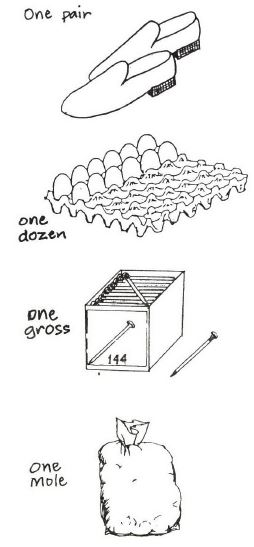
\includegraphics[width=0.4\textwidth]{./img/source/mole-concept.jpg}
\end{center}

\begin{description*}
%\item[Subtopic:]{}
%\item[Materials:]{}
%\item[Setup:]{}
%\item[Procedure:]{}
%\item[Hazards:]{}
%\item[Questions:]{}
%\item[Observations:]{}
\item[Theory:]{To show that 1 mole is a number of
particles or pieces, show that 1 pair = 2 pieces,
1 dozen = 12 pieces, 1 gross = 144 pieces, I mole = 6.022 $\times$ 10$^{23}$ particles.}
%\item[Applications:]{}
%\item[Notes:]{}
\end{description*}

\columnbreak

\subsection{Avogadro's Number}

%\begin{center}
%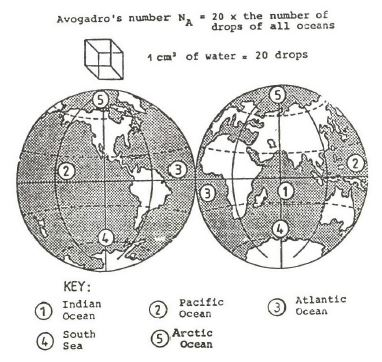
\includegraphics[width=0.49\textwidth]{./img/source/avogadro.jpg}
%\end{center}

\begin{description*}
%\item[Subtopic:]{}
%\item[Materials:]{}
%\item[Setup:]{}
%\item[Procedure:]{}
%\item[Hazards:]{}
%\item[Questions:]{}
%\item[Observations:]{}
\item[Theory:]{To illustrate the magnitude of Avogadro's
number the following comparison can be made:
If 1 cm$^3$ cube of water contains 20 drops of water
then Avogadro's number, N = 20 $\times$ the number of
drops in all the oceans of the world.}
%\item[Applications:]{}
%\item[Notes:]{}
\end{description*}

\subsection{Introducing Particle Masses}

\begin{center}
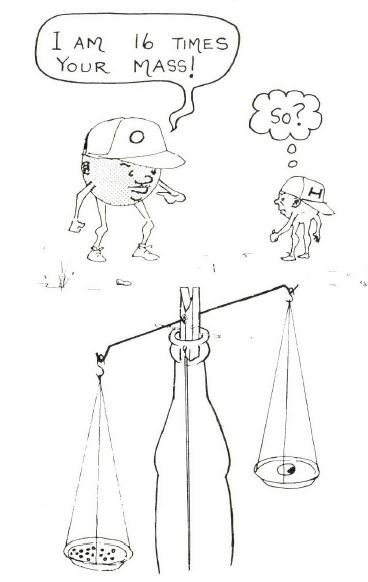
\includegraphics[width=0.4\textwidth]{./img/source/particle-mass.jpg}
\end{center}

\begin{description*}
%\item[Subtopic:]{}
\item[Materials:]{Balance, large seed, small seeds}
%\item[Setup:]{}
\item[Procedure:]{Take a balance and one stone/
big seed and weigh how
many other seeds make up the same weight. Make sure the objects are at the same distance
from the pivot.}
%\item[Hazards:]{}
%\item[Questions:]{}
%\item[Observations:]{}
\item[Theory:]{Different particles have different masses. The molar mass of a substance is a measure of the weight of a given number of particles of that substance. The standard number of particles used for comparing molar masses is a mol of particles (or 6.022 $\times$ 10$^{23}$).}
%\item[Applications:]{}
%\item[Notes:]{}
\end{description*}

\subsection{Understanding Atomic Mass}

\begin{center}
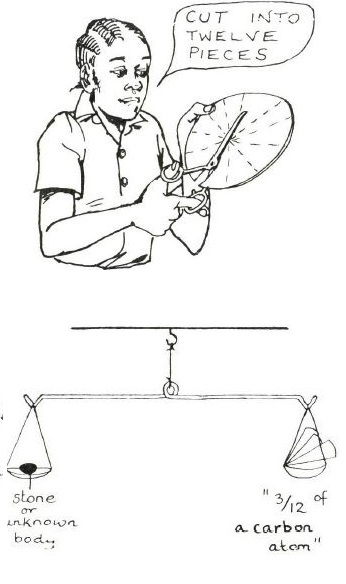
\includegraphics[width=0.4\textwidth]{./img/source/atomic-mass.jpg}
\end{center}

\begin{description*}
%\item[Subtopic:]{}
\item[Materials:]{Cardboard, scissors, balance}
%\item[Setup:]{}
\item[Procedure:]{Make a cardboard disc from thick cardboard. Divide into
12 parts and cut these out. One part represents
1/12, i.e. 1/12 of a carbon atom. Now try
to find out by weighing what the masses of
some unknown bodies are. These should be
heavier than 1 and not exceed 12 pieces.}
%\item[Hazards:]{}
%\item[Questions:]{}
%\item[Observations:]{}
\item[Theory:]{The mass of an object (atom) can be expressed relative to that of another. This is the concept behind molar mass. }
%\item[Applications:]{}
%\item[Notes:]{}
\end{description*}

\vfill
\columnbreak

\subsection{Molar Volume of Gases}

\begin{center}
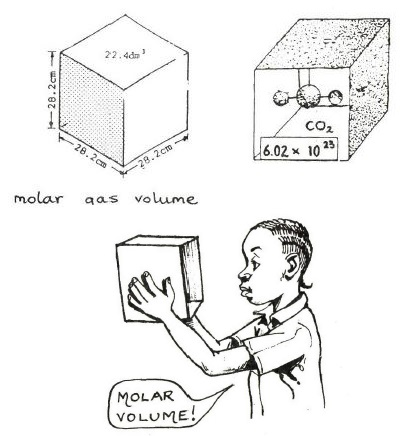
\includegraphics[width=0.45\textwidth]{./img/source/molar-volume.jpg}
\end{center}

\begin{description*}
%\item[Subtopic:]{}
\item[Materials:]{Cardboard, scissors, tape}
%\item[Setup:]{}
\item[Procedure:]{Cut out six 28.2 $\times$ 28.2 cm pieces of cardboard. Assemble them to form a cube of
volume 22.4 dm$^3$. Construct models of different
molecules and place/hang these in the box in
order to show that the 22.4 dm$^3$ volume is filled
with the same type and number of gas molecules.
Then write Avogadro's number and attach it to
the molecule model, and explain that in one
molar volume, there is that number of particles.}
%\item[Hazards:]{}
%\item[Questions:]{}
%\item[Observations:]{}
%\item[Theory:]{}
%\item[Applications:]{}
%\item[Notes:]{}
\end{description*}

\subsection{Molar Volume of Solids and Liquids}

\begin{center}
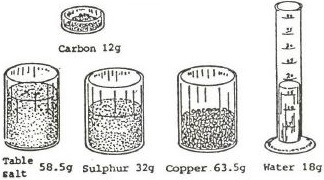
\includegraphics[width=0.45\textwidth]{./img/source/molar-volumes-2.jpg}
\end{center}

\begin{description*}
%\item[Subtopic:]{}
\item[Materials:]{Cups, water, various powders (e.g. carbon, sulphur, copper, salt)}
%\item[Setup:]{}
\item[Procedure:]{If you have a suitable balance, weigh out one
mole of various substances as shown in the
figure.}
%\item[Hazards:]{}
%\item[Questions:]{}
%\item[Observations:]{}
\item[Theory:]{The molar volume of different
solids and liquids is very different. Only the
molar volumes of gases - at the same temperature
and pressure - are the same.}
%\item[Applications:]{}
\item[Notes:]{To measure water, use 18 mL, since 1~mL $=$ 1~cm$^3$ and the density of water is about 1~g/cm$^3$.}
\end{description*}

\columnbreak

\subsection{Avogadro's Law}

\begin{center}
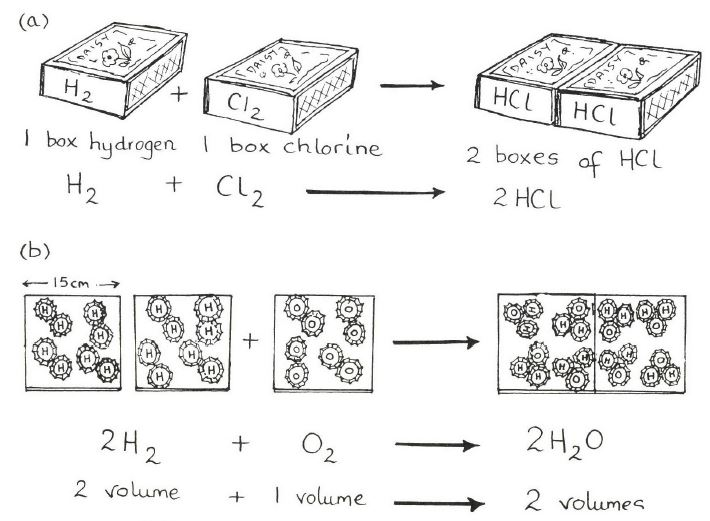
\includegraphics[width=0.49\textwidth]{./img/source/avogadro-law.jpg}
\end{center}

\begin{description*}
%\item[Subtopic:]{}
\item[Materials:]{Matchboxes, bottle caps}
%\item[Setup:]{}
%\item[Procedure:]{}
%\item[Hazards:]{}
%\item[Questions:]{}
\item[Observations:]{Each matchbox (all the same size) represents the same volume and each molecule in it the same number of particles.}
\item[Theory:]{Avogadro's Law states, that at the same
temperature and pressure equal volumes of
different gases contain the same number of
particles.}
\item[Applications:]{Chemical reactions may lead to same or different
volumes, e.g. in HCl and H$_2$O formation
respectively.}
%\item[Notes:]{}
\end{description*}

%==================================================================================================%

\section*{Dilution}


\subsection{Salt Dilution}

\begin{center}
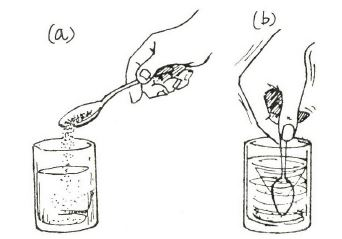
\includegraphics[width=0.4\textwidth]{./img/source/dilution.jpg}
\end{center}

\begin{description*}
%\item[Subtopic:]{}
\item[Materials:]{Salt, syringe, water, 5 bottles, food colour (optional)}
%\item[Setup:]{}
\item[Procedure:]{In one bottle, add 100 mL water and enough salt to saturate the solution. With a syringe remove 10 mL and add to another bottle with 90 mL of clean water. Now take 10 mL of this solution and add to another bottle with 90 mL of clean water. Repeat this several times, tasting a bit of each solution as you continue.}
%\item[Hazards:]{}
%\item[Questions:]{}
\item[Observations:]{The solution tastes less salty each time.}
\item[Theory:]{The ratio of solute to solvent (salt to water) decreases each time fresh water is added. Hence, the solution becomes more and more diluted.}
%\item[Applications:]{}
\item[Notes:]{Try also using food colour for a visual representation.}
\end{description*}

%\subsection{Colour Dilution}
%
%%\begin{center}
%%\includegraphics[width=0.4\textwidth]{./img/.jpg}
%%\end{center}
%
%\begin{description*}
%%\item[Subtopic:]{}
%\item[Materials:]{Water, food colour, syringe, 5 bottles}
%%\item[Setup:]{}
%\item[Procedure:]{Repeat the previous }
%\item[Hazards:]{}
%\item[Questions:]{}
%\item[Observations:]{}
%\item[Theory:]{}
%\item[Applications:]{}
%\item[Notes:]{}
%\end{description*}


\end{multicols}


\begin{center}
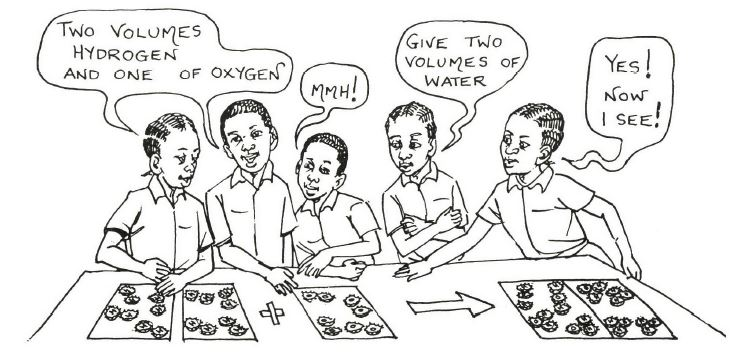
\includegraphics[width=0.9\textwidth]{./img/source/avogadro-students.jpg}
\end{center}

\pagebreak